\documentclass[11pt,a4paper]{article}

% Pacotes essenciais
\usepackage[utf8]{inputenc}
\usepackage[T1]{fontenc}
\usepackage{lmodern}
\usepackage[portuguese]{babel}
\usepackage{graphicx}
\usepackage{amsmath}
\usepackage{amsfonts}
\usepackage{amssymb}
\usepackage{float}
\usepackage{caption}
\usepackage{subcaption}
\usepackage{xcolor}
\usepackage{fancyhdr}
\usepackage{geometry}
\usepackage{titlesec}
\usepackage{lipsum}
\usepackage{cite}
\usepackage{booktabs}
\usepackage{array}
\usepackage{tikz}
\usepackage[hidelinks]{hyperref}

% Definição das cores
\definecolor{headercolor}{HTML}{b11116}
\definecolor{secondarycolor}{HTML}{3a5461}

% Configuração da página
\geometry{
    a4paper,
    top=2.8cm,
    bottom=2.5cm,
    left=2.5cm,
    right=2.5cm,
    headheight=1.2cm,
    headsep=0.5cm
}

% Configuração do cabeçalho
\pagestyle{fancy}
\fancyhf{}
\renewcommand{\headrulewidth}{0pt}
\renewcommand{\footrulewidth}{0.5pt}

\fancyhead[L]{%
    \begin{tikzpicture}[remember picture, overlay]
        \fill[headercolor] (current page.north west) rectangle ([yshift=-1.2cm]current page.north east);
        \node[anchor=west, inner sep=0pt] at ([xshift=1cm, yshift=-0.6cm]current page.north west) 
            {\includegraphics[height=0.8cm]{imgs/base/fatec-rgt.png}};
        \node[anchor=east, inner sep=0pt] at ([xshift=-1cm, yshift=-0.6cm]current page.north east) 
            {\includegraphics[height=0.9cm]{imgs/base/cps-logo.png}};
        \node[anchor=east, inner sep=0pt] at ([xshift=-2.8cm, yshift=-0.6cm]current page.north east) 
            {\includegraphics[height=1.05cm]{imgs/base/governo-sp-secretaria-logo.png}};
    \end{tikzpicture}
}

\fancyfoot[L]{\footnotesize\textcolor{secondarycolor}{Faculdade de Tecnologia do Estado de São Paulo\\ fatecregistro.cps.sp.gov.br}}
\fancyfoot[R]{\thepage}

% Configuração dos títulos das seções
\titleformat{\section}
    {\normalfont\large\bfseries\color{secondarycolor}}
    {\thesection}{1em}{}

\titleformat{\subsection}
    {\normalfont\normalsize\bfseries\color{secondarycolor}}
    {\thesubsection}{1em}{}

% Informações do artigo
\title{\vspace{0.6cm}\textbf{\Large Detecção de fungos parasitas em cogumelos usando aprendizagem profunda}}
\author{
    Andrei Araujo$^{1}$, Erlon Santos$^{2}$, Leandro Sueoka$^{3}$, Lucas Parada$^{4}$, Ricardo Estevam$^{5}$ \\[0.3cm]
    \small
    $^{1}$Faculdade de Tecnologia do Estado de São Paulo \\
    $^{2}$Fatec Registro \\[0.2cm]
    \begin{tabular}{c}
        \textit{andrei.araujo@aluno.cps.sp.gov.br} \\
        \textit{erlon.santos@aluno.cps.sp.gov.br} \\
        \textit{leandro.sueoka@aluno.cps.sp.gov.br} \\
        \textit{lucas.parada@aluno.cps.sp.gov.br} \\
        \textit{ricardo.estevam@aluno.cps.sp.gov.br}
    \end{tabular}
}
\date{}

\begin{document}

% Força o cabeçalho em todas as páginas
\pagestyle{fancy}

\maketitle
\thispagestyle{fancy}

% Resumo
\section*{Resumo}

\lipsum[0]Este trabalho apresenta um sistema inteligente de monitoramento para o cultivo de \textit{Pleurotus ostreatus} (shimeji), integrando sensores ambientais (temperatura, umidade e luminosidade) e visão computacional para detecção precoce de anomalias. A inteligência artificial baseia-se em aprendizagem profunda com a rede MobileNetV2, utilizando Transfer Learning a partir de pesos pré-treinados no ImageNet. O modelo foi treinado para classificação binária (saudável vs. anomalia), abrangendo fungos parasitas, estilamento e achatamento do chapéu, com 300 imagens divididas em 80\% para treino e 20\% para validação. Foram aplicadas técnicas de data augmentation e prevenção de overfitting, incluindo EarlyStopping, Dropout e class\_weight. Os resultados indicaram acurácia de 68,33\%, sensibilidade de 10\%, especificidade de 97,5\%, FPR de 2,5\% e FNR de 90\%. O modelo apresentou comportamento conservador, com alta especificidade e baixa sensibilidade na detecção de anomalias. Conclui-se que a integração entre IoT, visão computacional e aprendizagem profunda é promissora para a fungicultura, e que a coleta de mais dados e o ajuste do threshold podem melhorar o desempenho do sistema.
\vspace{0.3cm}
\noindent\textit{\textbf{Palavras-chave:}}  Aprendizagem Profunda; Cogumelos; Internet das Coisas.

\vspace{0.5cm}
\noindent\rule{\textwidth}{0.5pt}
\vspace{0.5cm}

% Introdução
\section{Introdução}

Os cogumelos constituem uma relevante fonte natural de nutrientes, destacando-se pelo elevado teor de proteínas, vitaminas e compostos bioativos benéficos à saúde humana. No mercado global de cogumelos comestíveis, as doenças fúngicas representam uma das principais causas de perdas produtivas. Esses organismos são cultivados predominantemente em ambientes fechados, sob condições ambientais controladas, o que favorece a adoção de programas integrados de manejo de doenças. Tais programas combinam o uso de fungicidas químicos, alternativas de biocontrole e práticas agronômicas adequadas, permitindo reduzir a incidência de patógenos e garantir o manejo sanitário das culturas. Dessa forma, diversos métodos de controle são continuamente aplicados com o objetivo de minimizar perdas e assegurar a qualidade do produto final \cite{Bellettini2017}.

Com base nesse cenário, a aplicação de tecnologias emergentes no setor agrícola possibilita o aumento da eficiência produtiva, a redução de perdas e a melhoria da qualidade dos alimentos e fatores diretamente relacionados à segurança alimentar. Além disso, o monitoramento contínuo de variáveis ambientais, como umidade e temperatura, permite otimizar o uso de recursos naturais, reduzir o desperdício de insumos e promover uma produção mais sustentável, resiliente e alinhada às demandas atuais por sistemas agrícolas inteligentes e ecologicamente responsáveis.

No contexto brasileiro, o \textit{Pleurotus ostreatus} (shimeji) destaca-se entre as espécies mais amplamente cultivadas, devido ao seu elevado valor nutricional e à crescente demanda no mercado alimentício. Entretanto, o aumento da produção tem sido acompanhado por uma maior ocorrência de contaminações microbiológicas, resultantes da proliferação de microrganismos oportunistas durante as etapas de cultivo e processamento, podendo ocasionar perdas totais nas colheitas. As infestações por pragas e doenças comprometem significativamente a qualidade e a composição do produto final, reduzindo a competitividade do produtor no mercado e impactando negativamente a rentabilidade e a sustentabilidade da produção \cite{Scheffer2023}.

Com isso, o Vale do Ribeira, localizado no Estado de São Paulo, destaca-se como uma região promissora para a implementação de sistemas baseados em tecnologias inteligentes. Essa região, foco da presente pesquisa, apresenta um constante crescimento na produção de espécies de cogumelos, especialmente o shimeji, o que reforça o potencial de aplicação de soluções tecnológicas voltadas ao monitoramento e controle de variáveis ambientais, contribuindo para o fortalecimento da produção local e o desenvolvimento sustentável do setor \cite{Urben2017}.

Ademais, a pesquisa de campo realizada com produtor local evidenciou demandas relacionadas ao acompanhamento automatizado da produção, principalmente no que se refere ao monitoramento das condições ambientais, à redução de perdas e à geração de relatórios. Tais aspectos corroboram a necessidade de ferramentas tecnológicas acessíveis e compatíveis com a realidade produtiva regional.

Apesar de a literatura contemplar investigações sobre monitoramento e aplicação de inteligência artificial (IA) no cultivo de cogumelos, os trabalhos disponíveis concentram-se, predominantemente, na classificação taxonômica de espécies ou na proposição de arquiteturas para vigilância ambiental. Tampouco se observa, no âmbito comercial, uma solução que conjugue esses dois domínios --- sensoriamento e IA --- e que se apresente como ferramenta operacional ao usuário final. Embora as produções científicas existentes apresentem bons resultados de detecção, carecem de resultados considerando-se a lacuna das condições reais de cultivo (\textit{reality gap}) observados na literatura \cite{Bennin2026}.

Entre os modelos de redes neurais existentes, a MobileNetV2 destaca-se como uma solução que combina baixo custo computacional e bom desempenho. Graças ao uso de convoluções \textit{depthwise} separáveis, seu custo computacional é de 8 a 9 vezes menor por camada em comparação às redes convolucionais tradicionais \cite{Sandler2018}. Dessa forma, a arquitetura torna-se adequada para aplicações em dispositivos com recursos limitados e pouco poder de processamento, como APIs hospedadas em servidores gratuitos ou sistemas embarcados.

Deste modo, o presente projeto tem como objetivo o desenvolvimento de um sistema inteligente de monitoramento do cultivo de cogumelos, voltado à prevenção de infecções e infestações por parasitas. A proposta visa integrar sensoriamento ambiental e IA para garantir o acompanhamento automatizado das condições do composto e do desenvolvimento dos cogumelos. O sistema será responsável por coletar e exibir dados em tempo real sobre umidade, temperatura e porcentagem estimada de infecção, obtidos por meio de sensores instalados no ambiente de cultivo, permitindo que o produtor acompanhe remotamente as condições ideais para o crescimento saudável dos fungos.

Além disso, será implementada uma IA baseada em aprendizagem profunda (\textit{deep learning}). As imagens capturadas no ambiente serão processadas e utilizadas tanto para o treinamento da IA quanto para o monitoramento contínuo do cultivo. O modelo será treinado para identificar padrões visuais indicativos de infecções e parasitas, como alterações de cor, presença de manchas e irregularidades no composto. Quando o sistema detectar anomalias que indiquem risco de contaminação, a porcentagem de alerta será automaticamente ajustada e o produtor será notificado por meio do aplicativo, permitindo uma resposta rápida e precisa no manejo das culturas.

Alinhando-se o presente estudo com a Agenda 2030 e os Objetivos de Desenvolvimento Sustentável (ODS) propostos pela Organização das Nações Unidas (ONU), a presente pesquisa relaciona-se diretamente ao ODS nº 2 --- Fome Zero e Agricultura Sustentável. Este objetivo visa erradicar a fome e promover sistemas alimentares produtivos, resilientes e ambientalmente responsáveis. Dessa forma, o desenvolvimento de um sistema inteligente de monitoramento e prevenção no cultivo de cogumelos contribui não apenas para o aumento da produtividade e da segurança alimentar, mas também para a redução do desperdício e o uso eficiente dos recursos naturais, reforçando o compromisso com práticas agrícolas sustentáveis e inovadoras.

% Objetivo
\section{Objetivo}

Com esta pesquisa, tem-se como principal objetivo desenvolver um sistema inteligente de monitoramento para o cultivo de cogumelos, utilizando sensores ambientais e inteligência artificial, a fim de prevenir infecções e infestações por parasitas, proporcionando maior controle, segurança e produtividade ao produtor, utilizando níveis de umidade, temperatura e índice de infecção. Além disso, como metas parciais visa-se:

\begin{itemize}
    \item Implementar uma integração eficiente entre o sistema proposto e a área de atuação dos produtores do Vale do Ribeira, ampliando o acesso e a disponibilidade de dados para o aprimoramento contínuo do modelo de inteligência artificial.
    \item Desenvolver a integração de câmeras e sensores de temperatura e umidade em um ambiente de Internet das Coisas (IoT) funcional, possibilitando a coleta automatizada de dados e o monitoramento em tempo real das condições ambientais do cultivo.
\end{itemize}

% Estado da Arte
\section{Estado da Arte}

Nos últimos anos, o uso de técnicas de \textit{machine learning} (ML) e visão computacional na agricultura tem se expandido significativamente, oferecendo soluções avançadas para monitoramento, classificação e colheita de produtos cultivados em ambientes controlados. Em especial para este estudo, a aplicação dessas técnicas no cultivo de cogumelos tem se mostrado promissora.

Diversos estudos têm explorado algoritmos de detecção de objetos para localizar cogumelos em imagens e determinar o estágio de crescimento, visando otimizar a colheita.

Nguyen et al. \cite{Nguyen2024} projetaram e implementaram uma arquitetura de Sistema de Informação de Agricultura Inteligente (SAIS) em três camadas --- Dispositivo, Edge e Nuvem --- para o cultivo de cogumelos ostra (\textit{Pleurotus} spp.) em estufa, integrando um sensor ambiental IoT combinado (temperatura, umidade relativa e CO\textsubscript{2}) a uma câmera de vigilância RGB para coleta automatizada de dados. Técnicas de baixo custo foram empregadas, incluindo armazenamento de pequenos dados, reamostragem temporal para redução de volume e controle de qualidade baseado em IA leve (algoritmo KNN com janela móvel de 24 h) para detecção de anomalias ambientais e lacunas em imagens. Também um modelo de \textit{deep learning} (YOLOv5), ajustado por \textit{transfer learning}, foi treinado para detecção de cogumelos e posteriormente implementado para inferência em tempo real, demonstrando que a integração de IoT sensorial, visão computacional e IA reduzem o tráfego de dados à nuvem e os custos operacionais, mantendo informações suficientes para o manejo automatizado do cultivo.

Outros estudos relevantes incluem a utilização do SSD (\textit{Single Shot MultiBox Detector}) em robôs colhedores de cogumelos, que alcançaram até 95\% de acurácia na detecção e 86,8\% de sucesso na colheita individual, evidenciando a viabilidade prática de sistemas automatizados em ambientes controlados \cite{Qian2020}. Pesquisas voltadas para a classificação de espécies de cogumelos comestíveis e venenosos mostraram que \textit{ensembles} de classificadores (Decision Tree, KNN, Random Forest, SVM, Naive Bayes) podem atingir 100\% de acurácia, reforçando a importância da inteligência artificial na diferenciação de cogumelos comestíveis e tóxicos \cite{Rahman2021}.

A integração de Internet das Coisas (IoT) com ML em sistemas de fungicultura inteligente também tem recebido destaque. Sensores de temperatura e umidade, associados a microcontroladores, permitem ajustar automaticamente variáveis críticas para o crescimento do micélio e do corpo de frutificação. Algoritmos de ML garantem a identificação precisa de cogumelos comestíveis, prevenindo a produção e consumo de exemplares tóxicos. Resultados experimentais indicam que esses sistemas mantêm condições ideais de temperatura e umidade, reduzem o esforço manual e fornecem dados em tempo real para os produtores. Avaliações de usabilidade (SUS) também demonstraram alto nível de satisfação, com pontuação média de 82\%, evidenciando a aplicabilidade prática dessas soluções \cite{Rahman2021}.

De forma complementar, Rahman et al. \cite{Rahman2021} demonstraram que a integração de sensores ambientais com sistemas IoT permite monitoramento contínuo em tempo real e emissão de alertas automáticos, garantindo respostas rápidas a alterações ambientais e promovendo uma gestão mais eficiente do processo produtivo.

Além disso, é possível encontrar na literatura sistemas que monitoram o crescimento e detectam doenças na produção de outras variedades de cogumelos. Nuankaew et al. \cite{Nuankaew2025} desenvolveram um sistema de monitoramento do cogumelo ostra focado na detecção de infecções causadas por fungos do gênero \textit{Trichoderma}, altamente contagiosos. Utilizando um sensor ótico e sensores de umidade e temperatura, o sistema coletava os dados que, por sua vez, eram avaliados por um algoritmo DenseNet201. Os resultados obtidos indicam acurácia de 92,50\% na detecção da doença em cogumelos. O estudo demonstra ser possível a utilização de tal sistema, permitindo que fungicultores possam tratar potenciais surtos, aumentando a eficiência da produção e reduzindo custos por perdas.

Desta forma, a integração entre algoritmos de aprendizagem profunda para análise visual, sensoriamento ambiental e tecnologias de Internet das Coisas (IoT) para monitoramento em tempo real configura uma abordagem tecnológica robusta e de elevada relevância para a produção de cogumelos. Soluções convencionais frequentemente apresentam restrições de acesso para usuários e produtores em campo, decorrentes de limitações de infraestrutura e da complexidade operacional. O sistema proposto neste projeto trata tais barreiras, viabilizando monitoramento remoto contínuo e fornecendo suporte automatizado à tomada de decisão. Essa abordagem estabelece uma base sólida para o desenvolvimento de sistemas inteligentes aplicáveis diretamente ao cultivo de espécies como o shimeji, promovendo incremento na produtividade, melhoria na segurança alimentar e maior sustentabilidade da fungicultura.

% Metodologia
\section{Metodologia}

Para a construção do sistema proposto, será implementada uma arquitetura de inteligência artificial baseada em aprendizado profundo (\textit{Deep Learning}), atuando como núcleo analítico do processo de monitoramento e detecção automatizada. O sistema integrará sensores óticos (câmeras com microcontrolador integrado) e sensores ambientais de temperatura, umidade relativa e luminosidade, interligados por uma infraestrutura IoT (\textit{Internet of Things}), responsável pela aquisição contínua e transmissão dos dados provenientes das estufas de cultivo.

Durante o processo de coleta, múltiplos fluxos de imagem (bloco 1) e dados ambientais (bloco 2) serão capturados em tempo real, encaminhados para o sistema via wi-fi (blocos 3 e 4), indexados e armazenados em um banco de dados não relacional (blocos 5 e 6), garantindo integridade e disponibilidade para uso posterior em tarefas de treinamento e validação de modelos.

O conjunto de imagens coletadas comporá o dataset primário para o treinamento supervisionado da IA. O modelo de aprendizado profundo, baseado em redes neurais, será configurado para detecção de padrões anômalos durante o crescimento, possibilitando a classificação automatizada dos estágios durante o desenvolvimento dos cogumelos e a identificação precoce de anomalias nos compostos.

Essa abordagem possibilita a criação de um sistema autônomo e adaptativo, capaz de realizar inferência em tempo real, monitorar o desenvolvimento dos cogumelos com alta precisão e fornecer alertas preditivos ao produtor sobre possíveis contaminações ou irregularidades no ambiente de cultivo.

\subsection{Desenvolvimento da Aprendizagem Profunda}

O processo de treinamento foi realizado utilizando \textit{Deep Learning}, com uma rede neural convolucional (CNN, tipo de rede neural para reconhecimento de padrões) da arquitetura MobileNetV2 (projetada para tarefas de visão computacional, ideal para dispositivos com recursos limitados) combinada a um MLP (\textit{Multi-Layer Perceptron}, rede neural com várias camadas de neurônios) para a classificação final. Para otimizar o processo de aprendizado, foi aplicada a técnica de \textit{Transfer Learning} (onde um modelo treinado é reutilizado em uma tarefa relacionada), reaproveitando os pesos pré-treinados no dataset ImageNet e congelando as camadas convolucionais, treinando apenas a cabeça de classificação.

A MobileNetV2 foi carregada com pesos pré-treinados no dataset ImageNet (um dos maiores e mais importantes bancos de imagens do mundo), e suas camadas convolucionais foram congeladas durante o treinamento inicial, atuando como extratoras de características visuais. Sobre ela, foi adicionada uma cabeça de classificação (onde as características extraídas nas camadas anteriores são traduzidas em previsão final) composta por:

\begin{itemize}
    \item \textbf{GlobalAveragePooling2D}\allowbreak: reduz a dimensionalidade dos mapas de características,\\resumindo-os em um único valor.
    \item \textbf{Camada Dense} (64 neurônios, ReLU): combina as características extraídas (gerando uma representação abstrata pronta para ser usada na decisão final).
    \item \textbf{Dropout} (0.5): previne overfitting (garantindo que a rede neural aprenda com os dados ao invés de memorizá-los).
    \item \textbf{Camada Dense} (1 neurônio, Sigmoid): saída binária (probabilidade de ser saudável).
\end{itemize}

A função de ativação Sigmoid foi utilizada na camada de saída, pois o problema é binário. A decisão final é tomada com base em um \textit{threshold} (limiar) ajustável (valores de 0.4, 0.5 e 0.6):

\begin{itemize}
    \item Se $probabilidade\_saudavel \geq threshold$ $\rightarrow$ Saudável
    \item Se $probabilidade\_saudavel < threshold$ $\rightarrow$ Anomalia
\end{itemize}

\subsection{Pré-processamento}

As imagens foram redimensionadas para 224x224 pixels e normalizadas (valores de pixel entre 0 e 1). Durante o treino, foi aplicado \textit{data augmentation} (aumento artificial do tamanho e diversidade do dataset) com:

\begin{itemize}
    \item Rotação (até 45°)
    \item Deslocamento horizontal e vertical (40\%)
    \item Cisalhamento (inclinação) de 30\%
    \item Zoom (40\%)
    \item Espelhamento horizontal
    \item Variação de brilho (0.5 a 1.5)
    \item Desfoque gaussiano (redução da nitidez) aleatório em 30\% das imagens
    \item Ruído gaussiano (simulação de imperfeições) em 20\% das imagens
\end{itemize}

Essas técnicas aumentaram artificialmente a diversidade do conjunto de treino, melhorando a capacidade de generalização do modelo.

\subsection{Treinamento}

O modelo foi compilado com o otimizador de aprendizagem Adam (taxa de aprendizado = 0.0001) e a função de perda \textit{binary crossentropy} (função para cálculo de perda). Foram utilizadas as seguintes técnicas de prevenção de overfitting:

\begin{itemize}
    \item \textbf{EarlyStopping} (monitorando \textit{val\_accuracy}, "paciência"), interrompendo o treinamento após 16, 25 e 50 épocas sem melhora na métrica monitorada;
    \item \textbf{ModelCheckpoint} (salvando o melhor modelo obtido ao término do EarlyStopping);
    \item \textbf{Class Weight} (utilizado em 9 testes para avaliar a compensação do desbalanceamento entre as classes devido à diferentes quantidades de fotos para treino).
\end{itemize}

O dataset foi dividido em 80\% para treino e 20\% para validação, com as seguintes quantidades de imagem por classe:

\begin{table}[ht]
\centering
\caption{Distribuição das imagens por classe}
\label{tab:distribuicao-imagens}
\begin{tabular}{lccc}
\hline
\textbf{Classe}   & \textbf{Treino} & \textbf{Validação} & \textbf{Total} \\ \hline
Saudável          & 80              & 20                 & 100            \\
Anomalia          & 160             & 40                 & 200            \\ \hline
\textbf{Total}    & \textbf{240}    & \textbf{60}        & \textbf{300}   \\ \hline
\end{tabular}
\end{table}

Como a classe ``Anomalia'' tinha o dobro de imagens da classe ``Saudável'', foi testado o \texttt{class\_weight='balanced'}, atribuindo peso maior à classe minoritária (saudável) durante o cálculo da perda.

\subsection{Fluxo de Processo}
Durante o funcionamento, o modelo treinado foi inserido em uma API desenvolvida em Python. Por sua vez, a API foi armazenada na plataforma de hospedagem Render utilizando o plano gratuito. O sistema executa o processamento em tempo real de imagem, capturando aproximadamente 1 frame por minuto. Cada frame é enviado ao modelo de IA, que realiza a inferência instantânea e gera uma estimativa probabilística de contaminação com base em características morfológicas detectadas (bloco 7). Quando um evento anômalo é identificado --- como a presença de fungos invasores ou alterações visuais atípicas --- o sistema gera alertas automáticos (blocos 8), notificando o produtor por meio do aplicativo integrado. Da mesma forma, os dados de avaliação da imagem são salvos no banco de dados. O software foi projetado para operar em uma aplicação mobile, destinada ao monitoramento em tempo real do ambiente de cultivo, exibição de alertas, acompanhamento de métricas de umidade, temperatura e iluminação, e consulta de painéis analíticos dinâmicos com gráficos de desempenho.

\begin{figure}[htb]
    \centering
    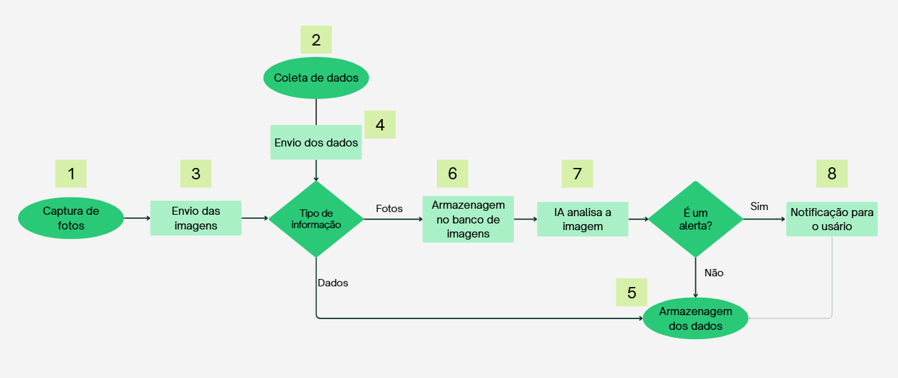
\includegraphics[width=\textwidth]{imgs/fluxograma.drawio.png}
    \caption{Fluxograma da metodologia adotada para desenvolvimento do sistema para detecção de parasitas em cogumelos}
    \label{fig:fluxograma}
    
    \vspace{2pt}
    {\small Fonte: Autoria própria, 2026}
\end{figure}

A comunicação entre as instâncias é realizada via API RESTful, permitindo sincronização contínua de dados e emissão de relatórios com informações sobre a saúde dos compostos, eficiência ambiental e status de contaminação. Essa integração garante que o produtor disponha de feedbacks em tempo real sobre o estado de suas produções e insumos preditivos para otimização de recursos e prevenção de perdas.

Como resultado, o sistema fornece uma plataforma inteligente e autônoma de monitoramento preditivo de fungicultura, combinando visão computacional, IoT e aprendizado profundo em uma arquitetura escalável, voltada à melhoria da produtividade, qualidade e sustentabilidade dos cultivos de \textit{Pleurotus ostreatus} (shimeji).

\subsection{Aplicação}
O backend da aplicação foi desenvolvido em Node.js com Express, em JavaScript. A API usa MongoDB via Mongoose, JWT para autenticação e Socket.IO para comunicação em tempo real. Para armazenamento de imagens é utilizado o Cloudinary.

O aplicativo mobile utiliza React Native com Expo e Expo Router, em TypeScript. Também utiliza Axios para chamadas à API, AsyncStorage para armazenamento local e módulos do Expo para notificações, áudio e outros recursos.

O hardware utilizado consiste em um microcontrolador ESP32 com sensores de temperatura, umidade e luminosidade e uma câmera ESP32 para registro das imagens.

% Resultados e Discussões
\section{Resultados e Discussões}

De acordo com as variáveis pre-estabelecidas (class weight, Early Stopping e  Threshold), foi definida uma matriz para os testes de treino dos modelos, conforme Tabela 2.

\begin{table}[htb]
\centering
\caption{Configurações de treinamento avaliadas}
\label{tab:configuracoes-treino}
\begin{tabular}{cccc}
\hline
\textbf{Treino} & \textbf{Class Weight} & \textbf{Early Stopping} & \textbf{Threshold} \\ \hline
1  & Sim & 16 & 0.4 \\
2  & Sim & 16 & 0.5 \\
3  & Sim & 16 & 0.6 \\
4  & Sim & 25 & 0.4 \\
5  & Sim & 25 & 0.5 \\
6  & Sim & 25 & 0.6 \\
7  & Sim & 50 & 0.4 \\
8  & Sim & 50 & 0.5 \\
9  & Sim & 50 & 0.6 \\ \hline
10 & Não & 16 & 0.4 \\
11 & Não & 16 & 0.5 \\
12 & Não & 16 & 0.6 \\
13 & Não & 25 & 0.4 \\
14 & Não & 25 & 0.5 \\
15 & Não & 25 & 0.6 \\
16 & Não & 50 & 0.4 \\
17 & Não & 50 & 0.5 \\
18 & Não & 50 & 0.6 \\ \hline
\end{tabular}
\end{table}

Desta forma, foram obtidos 18 modelos diferentes. Para avaliar o desempenho dos modelo obtidos, foram definidas métricas para avaliação pós-treinamento: acurácia (proporção total de acertos), sensibilidade (recall da anomalia, que mede a capacidade de detectar anomalias reais), especificidade (capacidade de identificar corretamente os casos saudáveis), taxa de falsos positivos (FPR, proporção de casos saudáveis classificados erroneamente como anomalia) e taxa de falsos negativos (FNR, proporção de anomalias classificadas erroneamente como saudáveis).

Para avaliar o desempenho dos modelos foram definidas métricas para avaliação pós-
treinamento: acurácia (proporção total de acertos), sensibilidade (recall da anomalia, que mede a capacidade de detectar anomalias reais), especificidade (capacidade de identificar corretament os casos saudáveis), taxa de falsos positivos (FPR, proporção de casos saudáveis classificados erroneamente como anomalia) e taxa de falsos negativos (FNR, proporção de anomalias classificadas erroneamente como saudáveis).
	
Nos primeiros 9 testes foram realizados treinos com balanceamento de classes (class weight, para avaliar se impacta no resultado do modelo), Early Stopping de 16, 25 e 50 (encerrando o treino de acordo com a quantidade de épocas sem evolução do modelo) e Threshould de 0.4, 0.5 e 0.6 (que é o limiar para definir se o resultado obtido com o modelo representa cogumelo com “anomalia” ou “saudável”. Os dados estão representados na figura 2.

\begin{figure}[H]
    \centering
    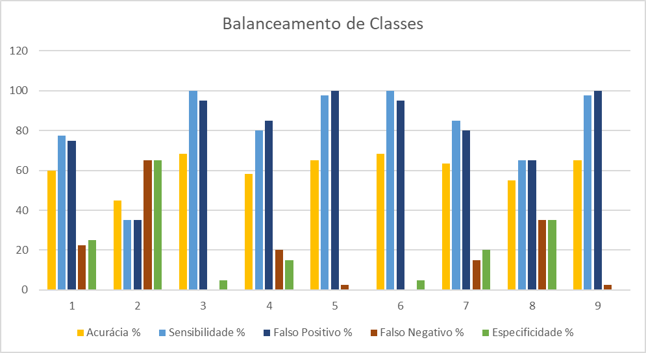
\includegraphics[width=\textwidth]{imgs/Fig2.png}
    \caption{Resultados obtidos com Balanceamento de classes}    
    \vspace{2pt}
    {\small Fonte: Autoria própria, 2026}
\end{figure}

Observa-se que os modelos treinados com \textit{class weight} apresentam resultados oscilantes, com acurácia entre 45 e 68,3\%, sensibilidade entre 35 e 100\%, especificidade entre 0 e 65\%, Falsos positivos entre 35 e 100\% e Falsos negativos entre 0 e 65\%. O treino 2 (realizado com Early Stopping de 16 e threshold de 0.5), embora tenha 45\% de acurácia, 35\% de sensibilidade e 65\% de especificidade, apresenta as métricas mais equilibradas de falsos positivos (35\%) e falsos negativos (65\%).

Os testes seguintes utilizaram as mesmas variáveis dos anteriores, porém sem o class weight. Os resultados obtidos estão na Figura 3.

\begin{figure}[H]
    \centering
    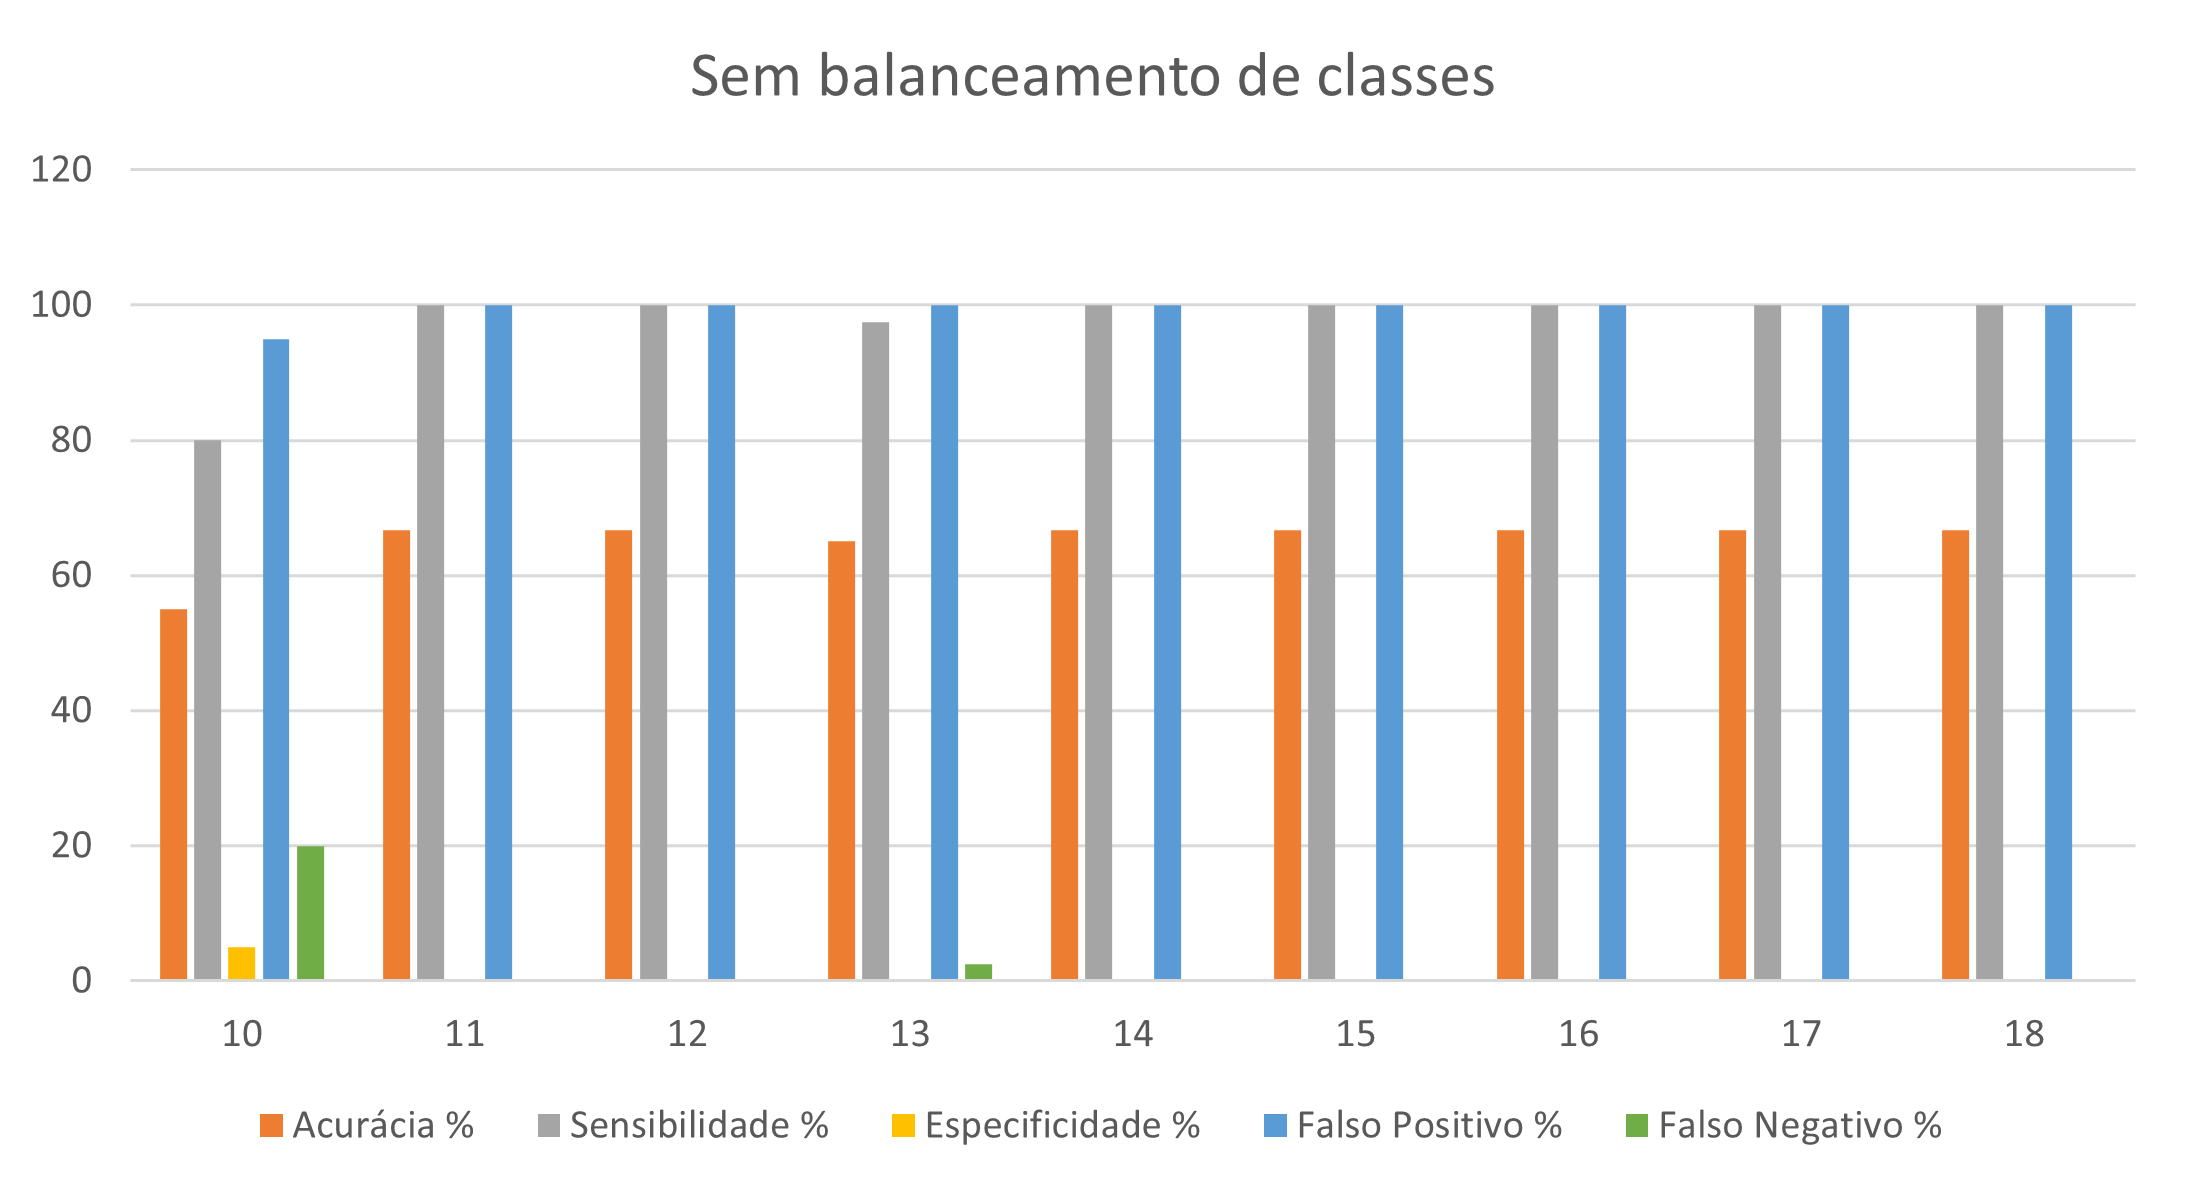
\includegraphics[width=\textwidth]{imgs/Fig3.png}
    \caption{Resultados obtidos sem balanceamento de classes}    
    \vspace{2pt}
    {\small Fonte: Autoria própria, 2026}
\end{figure}

Observa-se que os modelos treinados sem \textit{class weight} apresentam um padrão nos resultados, com falsos positivos acima de 95\% em todos os treinos. Desta forma, pode-se inferir que, mesmo as classes estando devidamente separadas para o treino do modelo (anomalia e saudável), as diferenças nas quantidades de imagens de cada classe impactam diretamente no desempenho do modelo, sendo que o balanceamento das classes fator determinante no desempenho do mesmo.


\subsection{Discussão}

O modelo, embora alcance resultados promissores, ainda apresenta uma baixa sensibilidade para diferenciação de cogumelos anômalos e saudáveis. Os resultados dos testes mostram que, mesmo nas melhores condições (conforme observado no treino 2 com class weight, Early Stopping de 16 e threshold de 0.5), ainda não obtiveram-se resultados satisfatórios de falsos positivos e falsos negativos simultaneamente baixos.

As principais causas identificadas foram:

\begin{itemize}
    \item \textbf{Dataset pequeno e pouco diversificado}: 100 imagens por classe, com muitas imagens visualmente semelhantes;
    \item \textbf{Desbalanceamento entre as classes}: a classe ``Anomalia'' tinha o dobro de imagens, o que foi compensado com \texttt{class\_weight}, mas ainda assim afetou o aprendizado;
    \item \textbf{Dificuldade inerente à tarefa}: algumas anomalias (especialmente fungos em estágio inicial) são visualmente sutis;
    \item \textbf{Baixa qualidade das imagens obtidas para o dataset}: as imagens fornecidas pela ESP32-CAM têm baixa resolução. Isso impacta diretamente no aprendizado e nos resultados do modelo proposto.
\end{itemize}

% Conclusão
\section{Conclusão}

O presente trabalho desenvolveu um sistema inteligente de monitoramento para o cultivo de Pleurotus ostreatus (shimeji), integrando sensores ambientais de temperatura, umidade e luminosidade a uma câmera ESP32-CAM em uma arquitetura IoT funcional. O sistema foi capaz de coletar dados ambientais e imagens de forma automatizada, transmiti-los via Wi-Fi e armazená-los em banco de dados não relacional, permitindo o monitoramento remoto em tempo real. A inteligência artificial, baseada em MobileNetV2 com Transfer Learning, foi integrada a uma API FastAPI, possibilitando a classificação automática de imagens em saudável ou anomalia (fungos, estilamento e achatamento). Os resultados obtidos no conjunto de validação indicaram modelos com variação nos resultados de classificação devido, principalmente, ao dataset reduzido. Conclui-se que a integração entre IoT, visão computacional e aprendizagem profunda é viável e promissora para a fungicultura do Vale do Ribeira, mas que o desempenho do modelo precisa ser aprimorado com a coleta de mais dados, ajuste do threshold de decisão e quantidade de épocas de treino. Como melhorias futuras, propõe-se a implantação do sistema em campo, a ampliação do dataset com mais imagens e a validação do índice de infecção junto aos produtores.

% Agradecimentos
\section*{Agradecimentos}

Os autores agradecem à Faculdade de Tecnologia do Estado de São Paulo (FATEC) e ao Centro Paula Souza (CPS) pelo apoio institucional.

% Referências
\bibliographystyle{IEEEtran}
\bibliography{referencias}

\end{document}
